\chapter{SUMMARY} 
This chapter presents results of the project, descriptions of its current state, achieved goals, our conclusions and future plans.

\section{Results (Jakub Kinder)}
\label{sec:results}
Through the course of this diploma project, we managed to complete most of our goals, notably we created a functional and visually pleasing PC building trainer for CAVE.
It possesses the desired core functionalities and is made in a fashion that allows it to be scalable which is important for future improvements.

In its current state, the developed application allows players to properly interact with provided PC components using Hand mechanics presented in \autoref{chap:ObjectHolding}.
Also, it possesses correct component connection mechanic described in \autoref{chap:ConnectingComponents} as well as progress tracking system, \autoref{chap:buildmanager}.
Furthermore, the trainer boasts helpful GUI elements in form of the clock measuring building time, task list, which guides novice PC builders through most common PC building procedure as well as information panel for each PC part, described in depth in \autoref{chap:GUI}.
The application, also features cables, that are essential part of PC building, however, due to their late appearance in the project they still need refinement.



\section{Conclusions}

\section{Future plans (Jakub Jędrzejczyk)}
\label{sec:FuturePlans}

\subsection{Bugfixes (Jakub Jędrzejczyk)}

Despite our best efforts to test the code before finalizing the release for user testing purposes, a few bugs have been identified that ought to be addressed, should work continue on this project.

The most glaring issue is the fact that the AMD CPU compatible motherboard's RAM slots fail to connect to any of the available RAM modules.
This is likely caused by misconfiguration of either of the problematic components' slot definitions, and should be relatively straightforward to fix.
% to się poprawi szybko i zmieni na czas przeszły

Another issue is that sometimes if a slot overlaps two slots (one valid, one invalid to place the part in), the connected component might end up attached to the invalid slot instead of the valid one, if the user decides to make the connection.
During testing, users were instructed to do their best to ensure a component's slot only overlapped a single, valid slot, but we recognize that this is not a viable, long-term solution.
This issue may stem from unexpected behavior in the event binding algorithm, and will require further investigation.
% tutaj pewnie obrazk z porównaniem dobrego i złego zachowania

While connections between components work as intended, there is a very rare bug in which the component being connected may end up moving not towards the slot it is being connected to, but rather towards the very centre of the target component (i.e. the parent of the target slot).
Given how otherwise reliable this functionality is, this may again be an issue in the event binding, as it appears as though the would-be parent is instead treated as the released component, making it the child of the connection.
% przykład, dobry byłby procesor który się połączył do środka płyty głównej zamiast do slotu

These are all the bugs that have been identified so far.
Whereas the first was easy to fix and has already been addressed, the other two will require further investigation and testing to ensure they are properly resolved.
Fortunately, none of these bugs make it impossible to use the application, though in the context of an otherwise polised product, they do detract from the overall user experience.
As known and documented issues, these would be the first to be addressed, should further development of the project be undertaken.

\subsection{Controller Joystick Rotation Fixes (Jakub Jędrzejczyk)}
\label{sec:ControllerJoystickRotationFixes}

The most raised issue by testers (as per subchapter \ref{sec:user-testing-results}) was the difficulty in rotating components using the joystick on the VR controllers.
While the development team found the rotation mechanics to be a helpful part of the building process, the users found it unintuitive and cumbersome, often leading to frustration and mistakes, requiring a lot of trial and error to get the desired orientation of components.
We believe this to be caused by the fact that most users chose this method of rotation over physically rotating their hands, and while a more in-depth tutorial on how to use the joystick rotation could help alleviate this issue, it may still be necessary to rework the rotation mechanics entirely.

The current implementation uses rotation axes fixed to the objects, which mean that a held object's rotation changes relative to its current orientation.
This means that if a user rotates an object 90 degrees on one axis, the other axes also change their orientation relative to the user, making further rotations possibly confusing.
A better approach would most likely be to use world space axes for rotation, meaning that no matter the current orientation of the object, pushing the joystick up would always rotate the object around the world's X axis, pushing it right would always rotate it around the world's Y axis.
Doing so would most likely require modification of the way a holdable object utilizes the RotatingMovement component, which by default uses local space axes for rotation.

Once done, this feature ought to be tested again with users to verify that the new rotation mechanics meet their expectations.

Additionally, it may be worth considering adding visual aids to help users understand the rotation mechanics better, particularly hinting about what direction the object should be rotated to fit into a slot.

\subsection{Data-driven components (Jakub Jędrzejczyk)}
\label{sec:DataDrivenComponents}

Originally, the available components were planned to be loaded dynamically using sets of files consisting of descriptions in JSON \cite{brayRFC8259JavaScript2017} format and model files.
The JSON files would contain all the necessary information about the object, such as its name, description, paths to the model files, specifications, component slots, their sizes, etc. 
The models would be in glTF 2.0 \cite{ISOIEC12113} format, which is a modern format for 3D models, supporting PBR materials and animations.

This approach allows for less coupling between the application and the content, and is an approach used in games such as Factorio, Sid Meier's Civilization, and, more recently, Minecraft (as many of the 2025 patches have focused on decoupling content from the core game engine).
% przydałyby się cytaty
This approach usually introduces higher up-front development time, as on top of the core functionality and content loading systems, tools for content creation and validation need to be developed.
The result, however, means that should development on the core application cease, users can freely extend the application's lifespan, even within the limits of existing functionality.

These plans were partially implemented, with a basic object loading system being created, but quickly deprioritized in favor of core functionality described previously.
Due to time constraints, the aforementioned tools for content creation and validation could not be created, with the current content being implemented entirely within Unreal Engine 5.

The planned functionality would require two blueprints - the first one would be responsible for scanning the folder with content in search of JSON files, while the second would spawn an object based on the description passed to it.
Each folder in the UserContent (made specifically for the purpose of allowing content to be edited by the User) directory would be treated as a category for objects to be sorted into (GPU, CPU, etc.).
% cytat potrzebny
Each one of these directories would then be read, and the object's description would be indexed within the application.
Given a wide selection of components, this would require relatively small memory footprint, with models and in-engine objects only being created on-demand, e.g. when a user selects a component from a list to be spawned in the scene.
The second blueprint would then load the model and create an appropriate object based on the description provided.

In the future, should this functionality be revisited, such a system could be implemented using serialization and deserialization techniques, allowing for usage of already implemented components as reference for future ones.

% \begin{figure}[H]
% 	\centering
% 		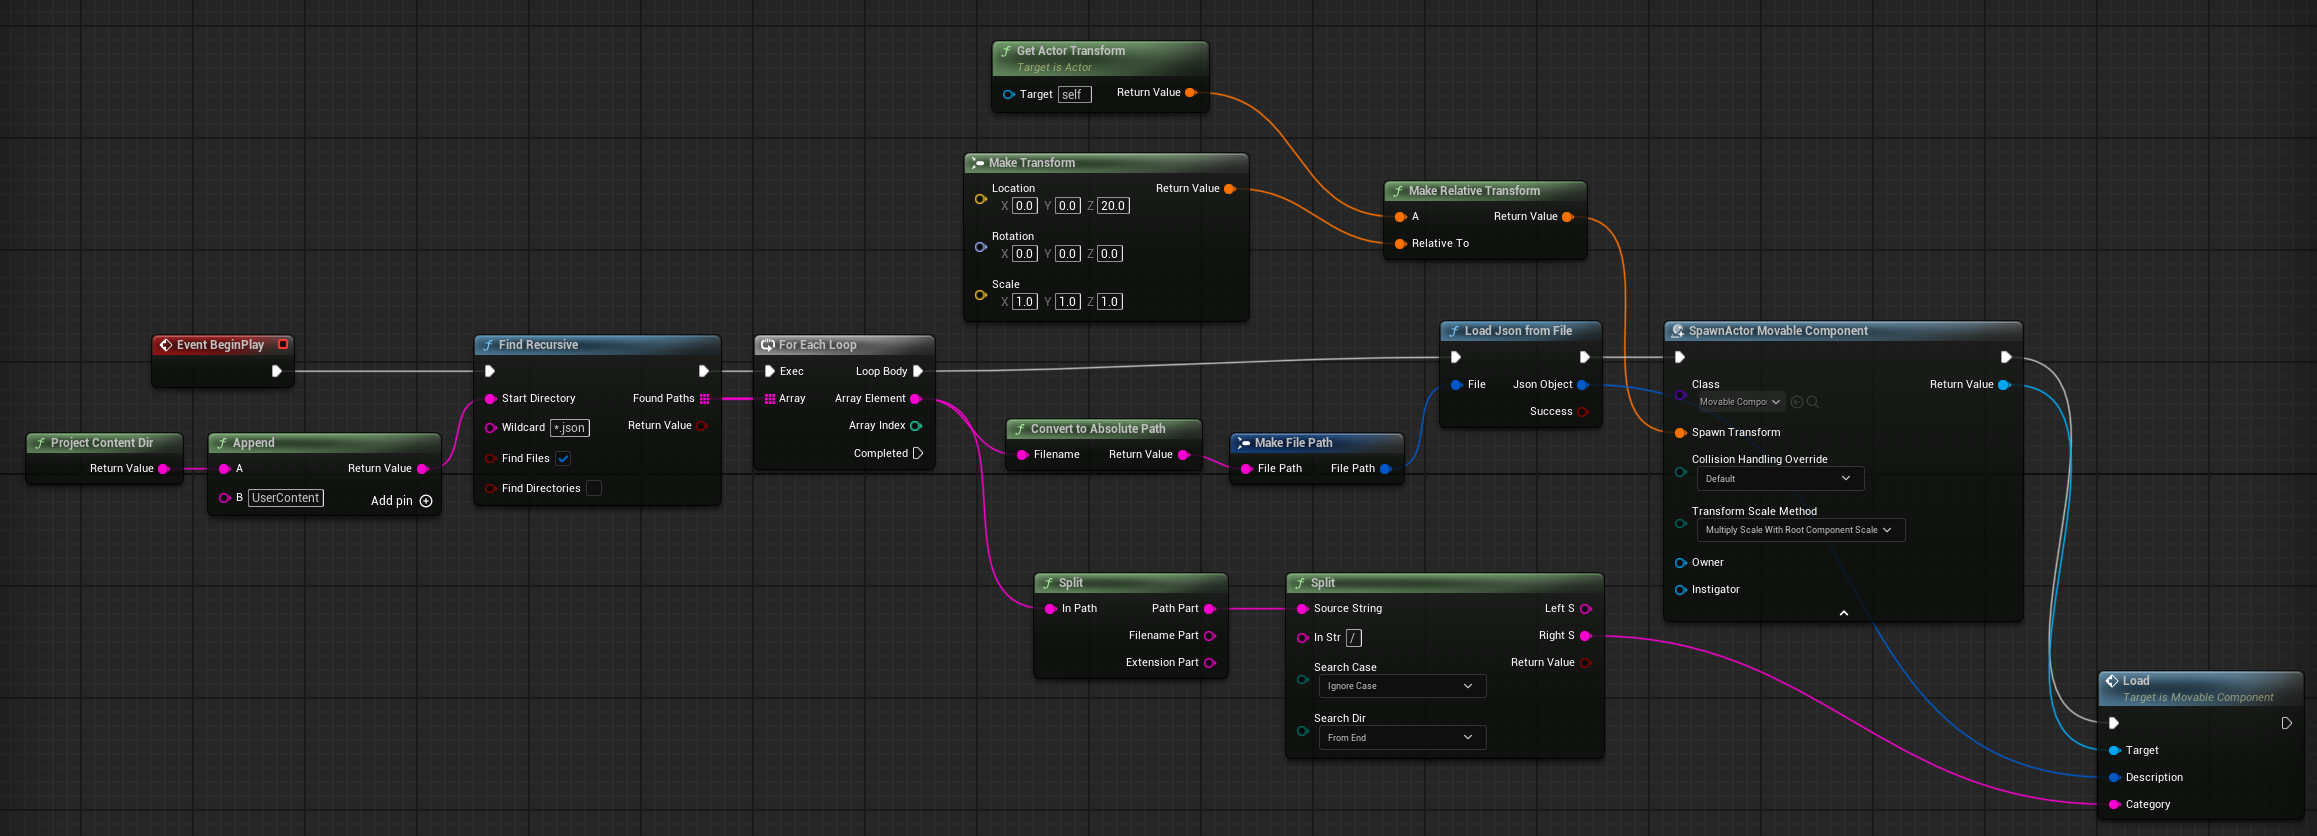
\includegraphics[width=1.0\textwidth]{Images/BasicLoadingBlueprint.png}
% 	\caption{Basic object loading blueprint}
% 	\label{fig:BasicLoadingBlueprint}
% \end{figure}

% The current loading scheme supports loading multiple meshes per object, which gives way to more complex models, such as GPUs with fans.
% Each mesh is expected to be a glTF 2.0 \cite{ISOIEC12113} model file, which is a modern format for 3D models, supporting PBR materials and animations.
% Each mesh can also be assigned a type, which is then used to assign specific functionality to it.
% For example, a mesh of type "Body" is treated as the main mesh of the object, while a mesh of type "Fan" could be rotated when the computer is turned on.

% \begin{figure}[H]
% 	\centering
% 		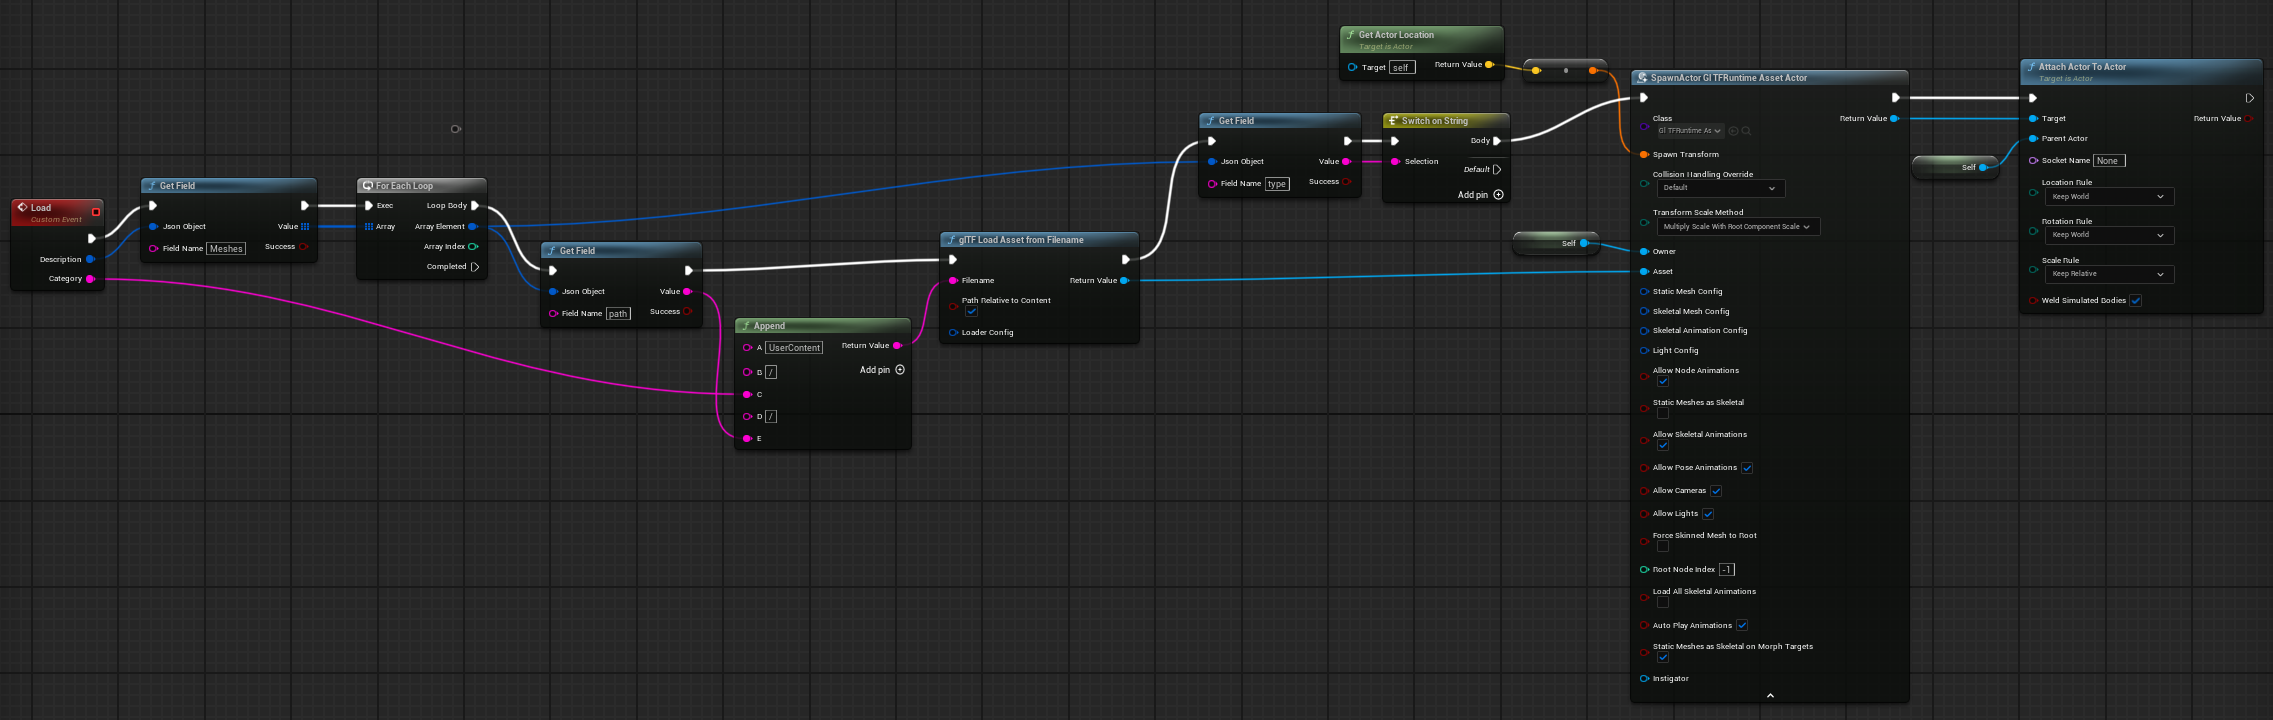
\includegraphics[width=1.0\textwidth]{Images/BasicObjectSelfPreparation.png}
% 	\caption{Basic object self-preparation blueprint}
% 	\label{fig:BasicObjectSelfPreparation}
% \end{figure}

% After placing this loading object in the scene and preparing appropriate description and model files, the object could be spawned in the scene at runtime.

% \begin{figure}[H]
% 	\centering
% 		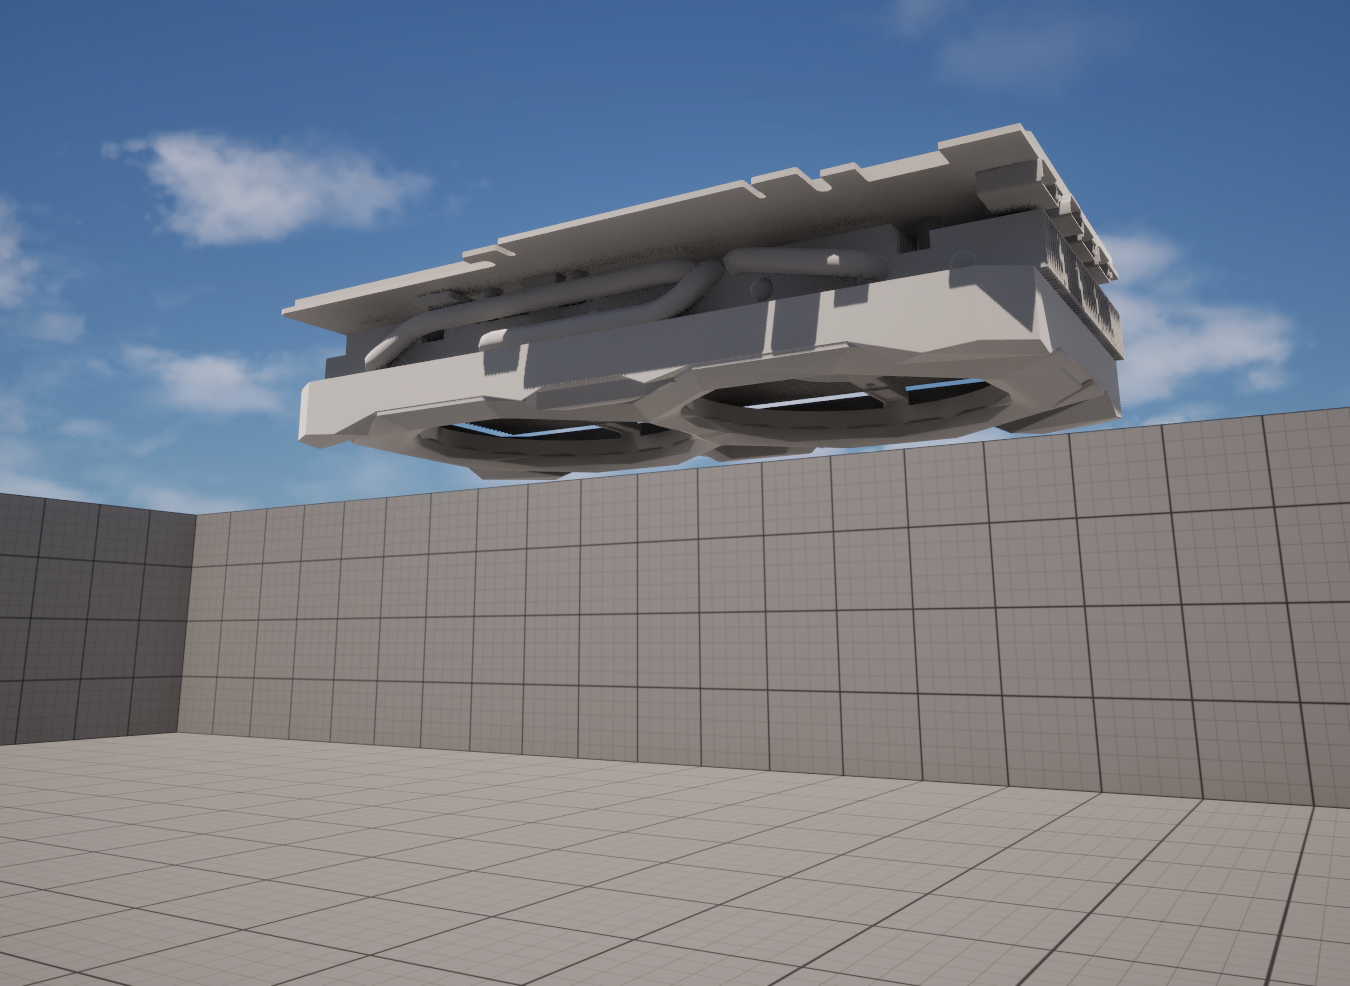
\includegraphics[width=0.7\textwidth]{Images/BasicGPULoaded.png}
% 	\caption{Basic GPU loaded blueprint}
% 	\label{fig:BasicGPULoaded}
% \end{figure}

\subsection{Wider Component Variety (Jakub Jędrzejczyk)}

\subsection{User Settings (Jakub Jędrzejczyk)}

\subsection{Detailed Interactions (Jakub Jędrzejczyk)}

While the current implementation of object interactions in the application is functional and allows users to complete the tasks at hand, there is room for improvement in terms of detail and realism.
Connecting components currently involves simply bringing them close enough to their respective slots, and letting go, at which point they snap into place.

To enhance the realism and immersion of the experience, more detailed interactions could be implemented.
For example, before installing a CPU into its socket, the user would be required to lift the socket lever, remove the protective cover, at which point they could place the CPU into the socket, ensuring it is properly aligned with the notches.
Once in place, the user would then need to lower the lever back down to secure the CPU, otherwise it could fall out during subsequent interactions, nullifying the installation.

Analogously, disconnecting components currently requires pressing a button, then picking up an object, which removes the connection.
A more detailed version of this interaction could involve the user needing to first lift a retention clip or unscrew screws securing the component in place, before being able to safely remove it.

Ideally, together with these features the screws and screwdriver which exist within the game should be fully functional, allowing users to screw and unscrew components as they would in real life.